\documentclass[a4paper, 12pt]{article}

\usepackage{mathtext}
\usepackage{cmap}
\usepackage[T1,T2A]{fontenc}
\usepackage[utf8]{inputenc}                                     
\usepackage[english,ukrainian]{babel}
\usepackage{graphicx}

\begin{document}

\begin{center}
    \textbf{Розрахункова робота №3}

    \textbf{Згасаючі або вимушені коливання}
\end{center}

\begin{flushright}
    Варіант 4

    Шкаліков Олег, ФІ-81
\end{flushright}

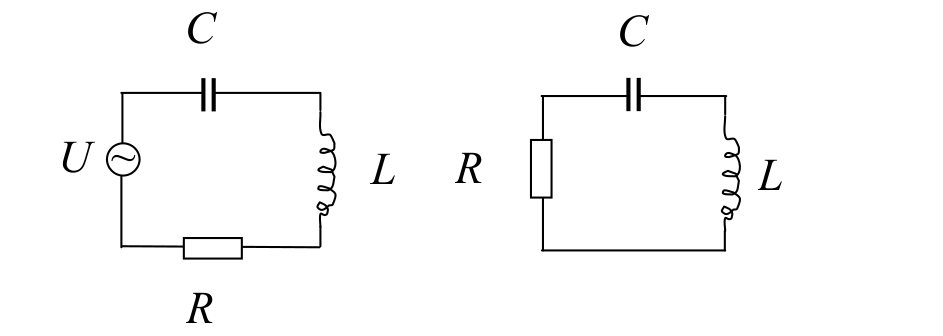
\includegraphics[width=1.0\textwidth]{graphics/RLC.png}
На малюнках зображено коливальний $RLC$ контур, для якого відомі:
власна колова частота $\Omega_0 = (LC)^{-1/2} = 235.7(c^{-1})$ за відсутності опору;
опір $R = 2$(Ом); критичний опір $R_{crit} = 9,4$(Ом). 
Генератор створює змінну напругу $\varepsilon  = \varepsilon_0 \cos{2\pi \nu t}$
з фіксованою амплітудою $\varepsilon_0 = 1$(В) та регульованою частотою $\nu = 30$(кГц). 
В подальшому позначимо $\omega \equiv 2 \pi \nu$.

\begin{enumerate}
    \item За відомими формулами знайти для контуру $RLC$ індуктивність $L$, 
    ємність $C$, коефіцієнт згасання, добротність $Q$.
    
    Запишемо рівняння для контура без генератора:
    $$ L\ddot{q} + R\dot{q} + \frac{q}{C} = 0 $$
    $$ 2\gamma = \frac{R}{L}, \; \Omega_0^2 = \frac{1}{LC} $$
    $$ \ddot{q} +  2\gamma \dot{q} + \Omega_0^2 q = 0 $$
    Характеристичне рівняння:
    $$ \lambda^2 + 2 \gamma \lambda + \Omega_0^2 = 0 $$
    $$ D = 4 \gamma^2 - 4 \Omega_0^2 = 2 \sqrt{\gamma^2 - \Omega_0^2}$$

    Коливання швидко не згасають за умови $\gamma^2 - \Omega_0^2 < 0$, 
    тобто коплексності дискримінанта. Отже:
    $$ D = 2i\sqrt{\Omega_0^2 - \gamma^2}, \; \omega^2 = {\Omega_0^2 - \gamma^2}$$
    $$ \lambda = \gamma \pm \omega $$
    $$ q(t) = e^{\gamma} \left( c_1 e^{\omega t} - c_2 e^{-\omega t} \right) $$

    $R_{crit}$ за визначенням дорівнює опору, за якого $D$ = 0, отже:
    $$D = 0 \Rightarrow \Omega_0 = \gamma 
    \Rightarrow L = \frac{R_{crit}}{2 \Omega_0} \simeq 20 (мкГн)$$
    
    Тоді маємо, що:
    $$ C = \frac{1}{\Omega_0^2 L} \simeq 0.9 (мкФ),\; 
    \gamma = \frac{R}{2L} \simeq 50149 (\frac{Ом}{Гн}),\; 
    Q = \frac{\Omega_0}{2 \gamma} \simeq 2.35$$

    \item Скласти диференціальне рівняння коливального контура з генератором.
    
    Надалі, для зручності, передемо у комплексну площину.

    $$ L\ddot{q} + R\dot{q} +  = \varepsilon_0 e^{i \omega t} $$
    $$ L\dot{I} +  RI + \frac{\int I dt}{C} = \varepsilon_0 e^{i \omega t} $$

    \begin{equation} \label{eq:RLC}
        L\ddot{I} +  R\dot{I} + \frac{I}{C} = i \omega \varepsilon_0 e^{i \omega t}
    \end{equation}    

    \item З рівняння отримати вираз для $I_0=I_0(\omega)$, тобто залежність
    амплітудного значення струму в контурі від частоти генератора.

    Представимо розв'язок рівняння \ref{eq:RLC} у вигляді $I(\omega) = I_0 e^{iwt+i\varphi}$. Тоді:
    $$ -L \omega^2 I_0 e^{iwt + i \varphi} + i \omega R I_0 e^{iwt + i \varphi} + \frac{I_0 e^{i \omega t + i \varphi}}{C} = i \omega \varepsilon_0 e^{i \omega t} $$
    $$ L \omega I_0 e^{i \varphi} + R I_0 e^{i \varphi} + \frac{I_0 e^{i\varphi}}{i \omega C} = \varepsilon_0 $$
    $$ I_0 = |I_0 e^{i \varphi}| = \frac{\varepsilon_0}{\sqrt{R^2 + \left( L \omega - \frac{1}{\omega C} \right)^2}} $$

    \item Отримати вираз та розрахувати значення резонасної колової частоти 
    $\omega_{res}$ та максимальної амплітуди струму $I_{0_{max}}(\omega_{res})$ в контурі.

    $$ \frac{dI_0}{d\omega} = 
    \frac{1}{2} \frac{2 \varepsilon_0 \left( L \omega- - \frac{1}{\omega C} \right) \left( L + \frac{1}{C \omega^2} \right)}
    { \left(R^2 + \left( L \omega - \frac{1}{\omega C} \right)^2 \right)^{\frac{3}{2}} }$$
    $$ \frac{dI_0}{d\omega} = 0 \Rightarrow \left( L \omega - \frac{1}{\omega C} \right) = 0 \Rightarrow 
    \omega_{res} = \frac{1}{\sqrt{LC}} = \Omega_0 $$
    $$ I_o(\omega_{res}) = \frac{\varepsilon_0}{R} = 0.5 (A)$$

    \item В інтервалі $\omega \in \left[ 0,2\Omega_0 \right]$ задати 20
    значень колової частоти генератора і побудувати графік $I_0=I_0(\omega)$.
    Одиниці вимірювання підібрати таким чином, щоб ціна найменшоб поділки на осях
    відповідала одиницям або десяткам. Вказати числові значення резонасної частоти
    та резонасної амплітуди струму.
    
    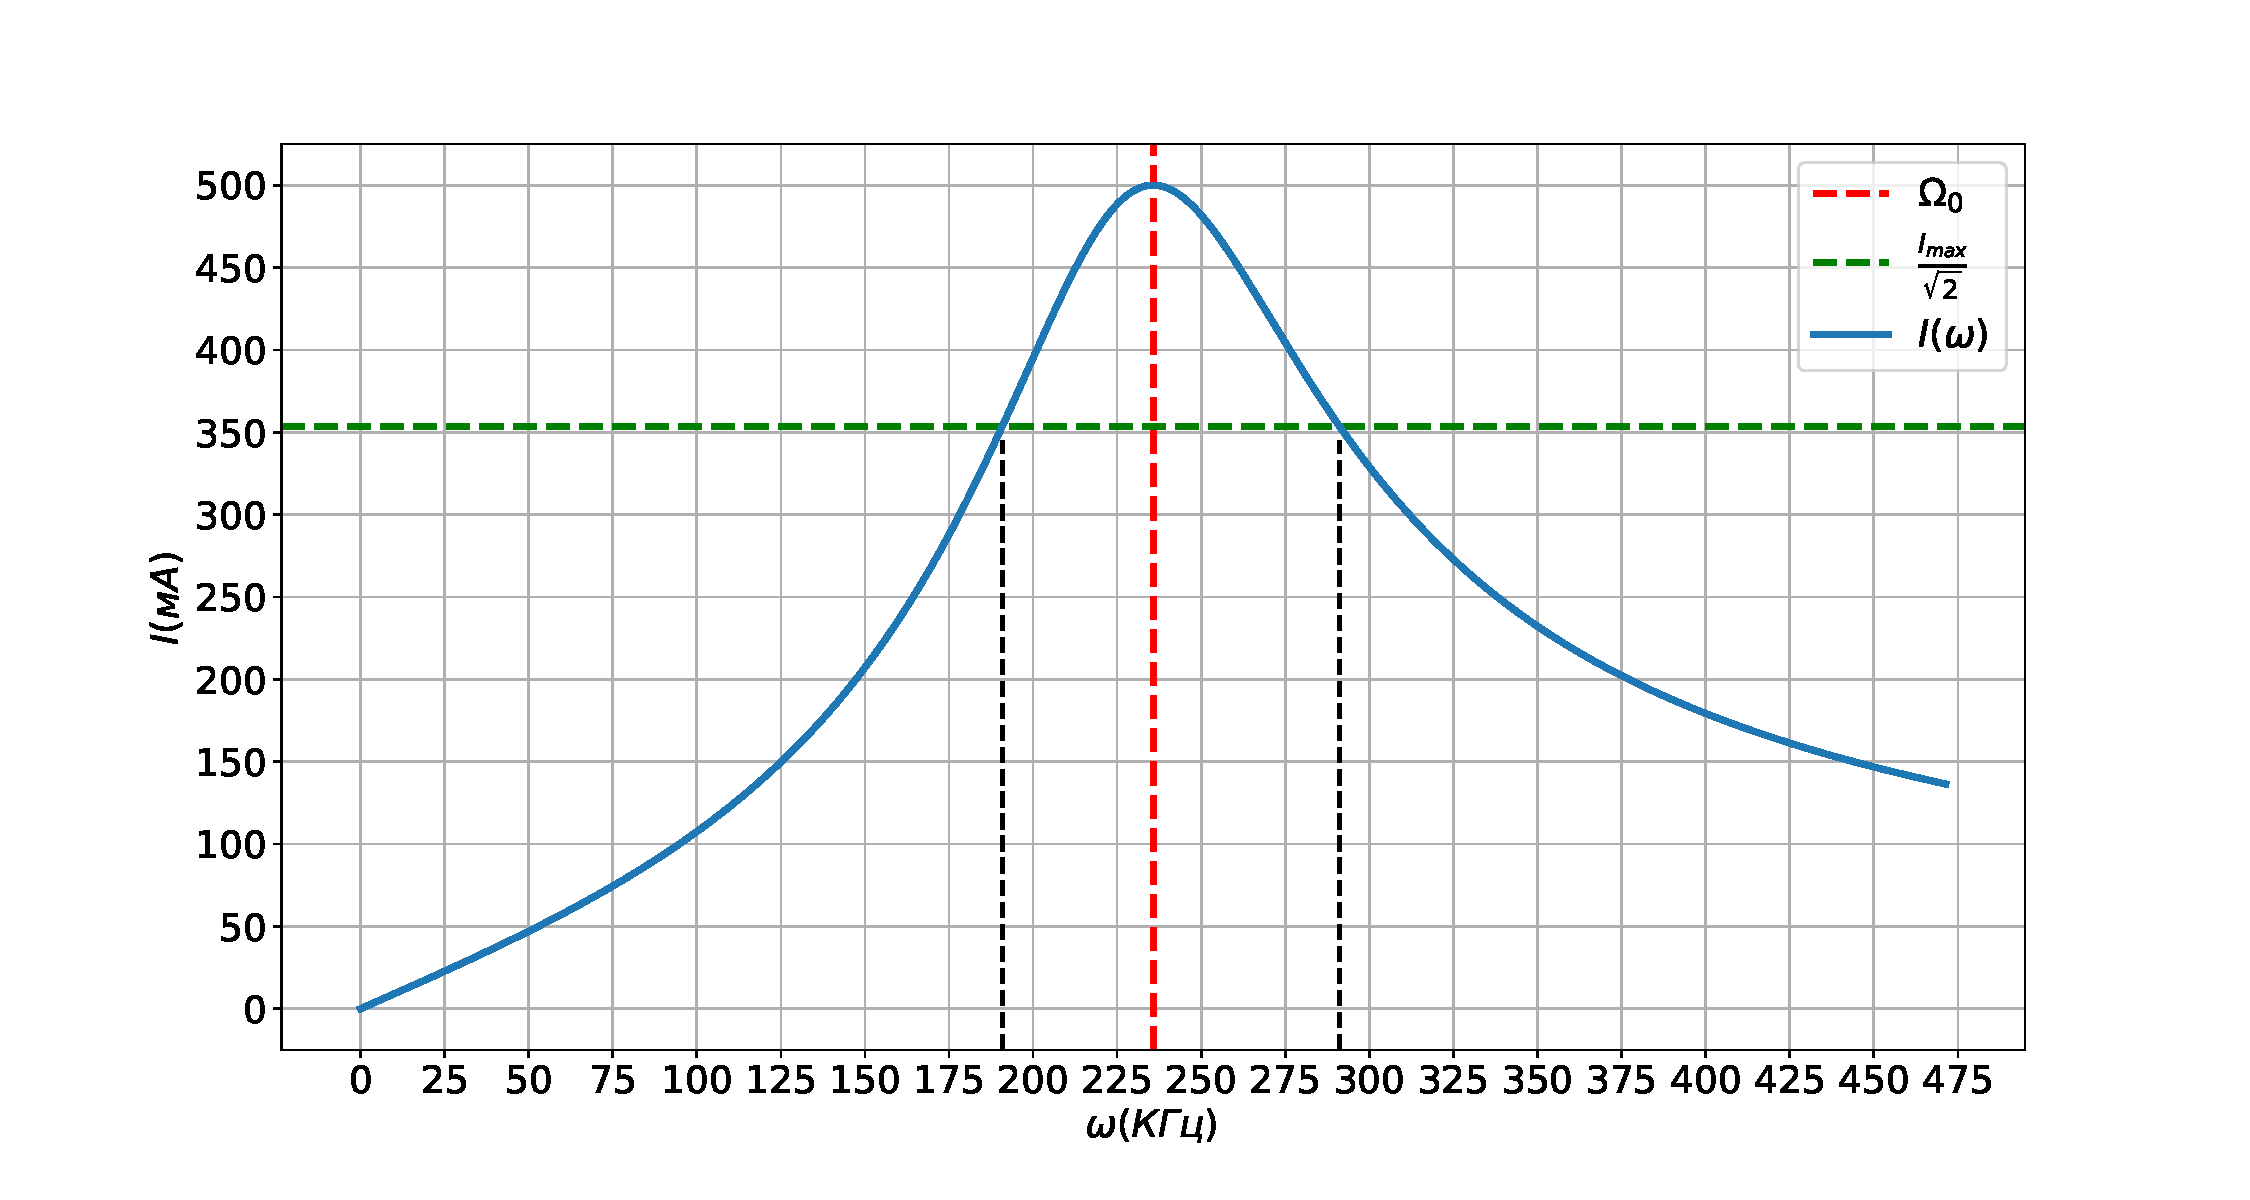
\includegraphics[width=1.0\textwidth]{graphics/I(w).pdf}

    \item За графіком знайти "експериментальне значення" добротності
    $$Q_* = \frac{\Omega_0}{\Delta \Omega}$$,
    де $\Delta \Omega$ визначається як різниця частот, при яких амплітуда
    струму дорівнює $I_{0_max}/\sqrt{2}$. 
    Визначити похибку $\eta = 100\% \left( Q-Q_* \right) / Q$.
 
    З графіку визначимо $\Delta \Omega = 98 \times 10^3(c^{-1})$, тоді:
    $$ Q_* \simeq 2.4, \; \eta \simeq 2.3 \%$$

    \item Розрахувати імпеданс контура на частоті $\nu$.

    $$ Z = \sqrt{R^2 + \left( 2 L \pi \nu - \frac{1}{2 \pi \nu C} \right)^2} \simeq 3(Ом)$$

    \item Розрахувати зсув фази $\varphi$ між струмом та напругою на генераторі(при частоті $\nu$).
    
    $$ \varphi = \arctan{\frac{Im{z}}{Re{z}}} = \arctan \frac{2 L \pi \nu - \frac{1}{2 \pi \nu C}}{R} \simeq -0.81(рад) \simeq -46^o $$
    
    \item Розрахувати діючі значення $I_g, \; \varepsilon_g$ струму та напруги і
    обчислити потужність, яку споживає контур:
    $$\langle P \rangle = \varepsilon_g I_g \cos{\varphi}$$

    $$ I_g = \frac{I_{0_{max}}}{\sqrt{2}} \simeq 0.35(А),\; 
    \varepsilon_g = \frac{\varepsilon_{0_{max}}}{\sqrt{2}} \simeq 0.7(В)$$
    $$ \langle P \rangle \simeq  0.17(Вт)$$

    \item Побудувати векторну діаграму кола на частоті $\nu$ та
    з'ясувати, яким навантаженням(ємнісним чи індуктивним) є коло генератора.
    
    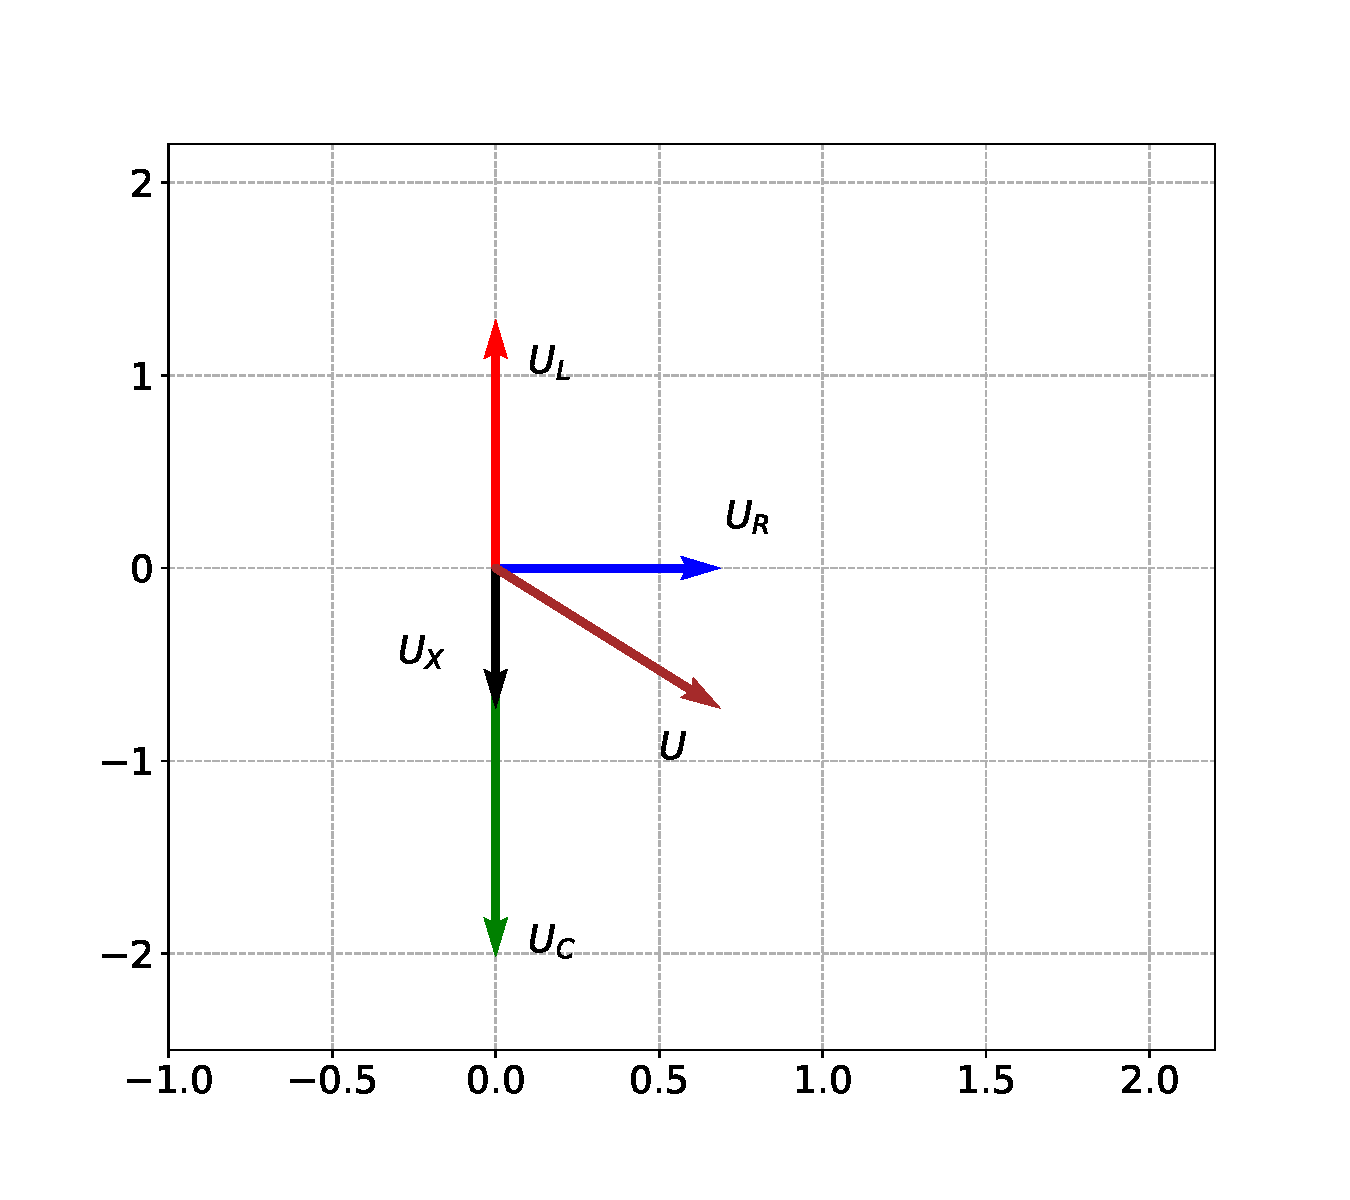
\includegraphics[width=0.8\textwidth]{graphics/vectorDiagramm.pdf}


    $U_L < U_C \Rightarrow$ розглянутий контур є ємнісним навантаженням.

    \item З рівняння контура отримати вираз для залежності $\varepsilon_C(\omega)$ 
    амплітуди напруги на конденсаторі від колової частоти генератора.
    
    $$ \varepsilon_C = |U_C| = |Z_C I_0| = \frac{I_0}{\omega C} =  \frac{\varepsilon_0}{\omega C\sqrt{R^2 + \left( L \omega - \frac{1}{\omega C} \right)^2}} $$

    \item Отримати вираз та обчислити резонасну колову частоту $\omega_{res}^{'}$ та
    резонасну амплітуду $\varepsilon_{C_{max}}(\omega_{res}^{'})$ напруги на конденсаторі.
    Визначити, наскільки відсотків $\omega_{res}^{'}$ відрізняється від власної частоти контура $\Omega_0$.
    
    $$ \frac{d \varepsilon_C}{d\omega} = \frac{I_0^{'} \omega C - C I_0}{(\omega C)^2} = 
    \frac{\frac{\varepsilon_0 \left( L \omega - \frac{1}{\omega C} \right) \left( L + \frac{1}{C \omega^2} \right) \left( \omega C  \right)}
    { \left(R^2 + \left( L \omega - \frac{1}{\omega C} \right)^2 \right)^{\frac{3}{2}} } - \frac{C \varepsilon_0}{\sqrt{R^2 + \left( L \omega - \frac{1}{\omega C} \right)}} } {\left( \omega C \right)^2} = $$
    
    $$ \frac{\varepsilon_0 \left( L \omega - \frac{1}{\omega C} \right) \left( L + \frac{1}{C \omega^2} \right) \left( \omega C  \right) - C \varepsilon_0 \left(R^2 + \left( L \omega - \frac{1}{\omega C} \right)^2 \right) }
    {\left( \omega C \right)^2 \left(R^2 + \left( L \omega - \frac{1}{\omega C} \right)^2 \right)^{\frac{3}{2}}} $$
    
    $$ \frac{d \varepsilon_C}{d\omega} = 0 \Rightarrow 
    \left( L \omega - \frac{1}{\omega C} \right) \left( L \omega + \frac{1}{\omega C} \right) -
    R^2 - \left( L \omega - \frac{1}{\omega C} \right)^2 = $$ 
    $$ L^2 \omega^2 - \frac{1}{\omega^2 C^2} + R^2 + L^2 \omega^2 - \frac{2L}{C} + \frac{1}{\omega^2 C^2} =
    2 L^2 \omega^2 + R^2 - \frac{2L}{C} = 0 $$ 
    
    $$ \Rightarrow \omega^2 = \Omega_0^2 - 2\gamma^2 \Rightarrow \omega_{res} = \sqrt{\Omega_0^2 - 2\gamma^2} $$
    
    Таким чином:
    $$ \omega_{res} \simeq 225\times10^3(c^{-1}),\; \varepsilon_{C_{max}}(\omega_{res}^{'}) = 2.4(B)$$

    \item Побудувати амплітудну характеристику напруги на конденсаторі $\varepsilon_C = \varepsilon_C(\omega)$.
    
    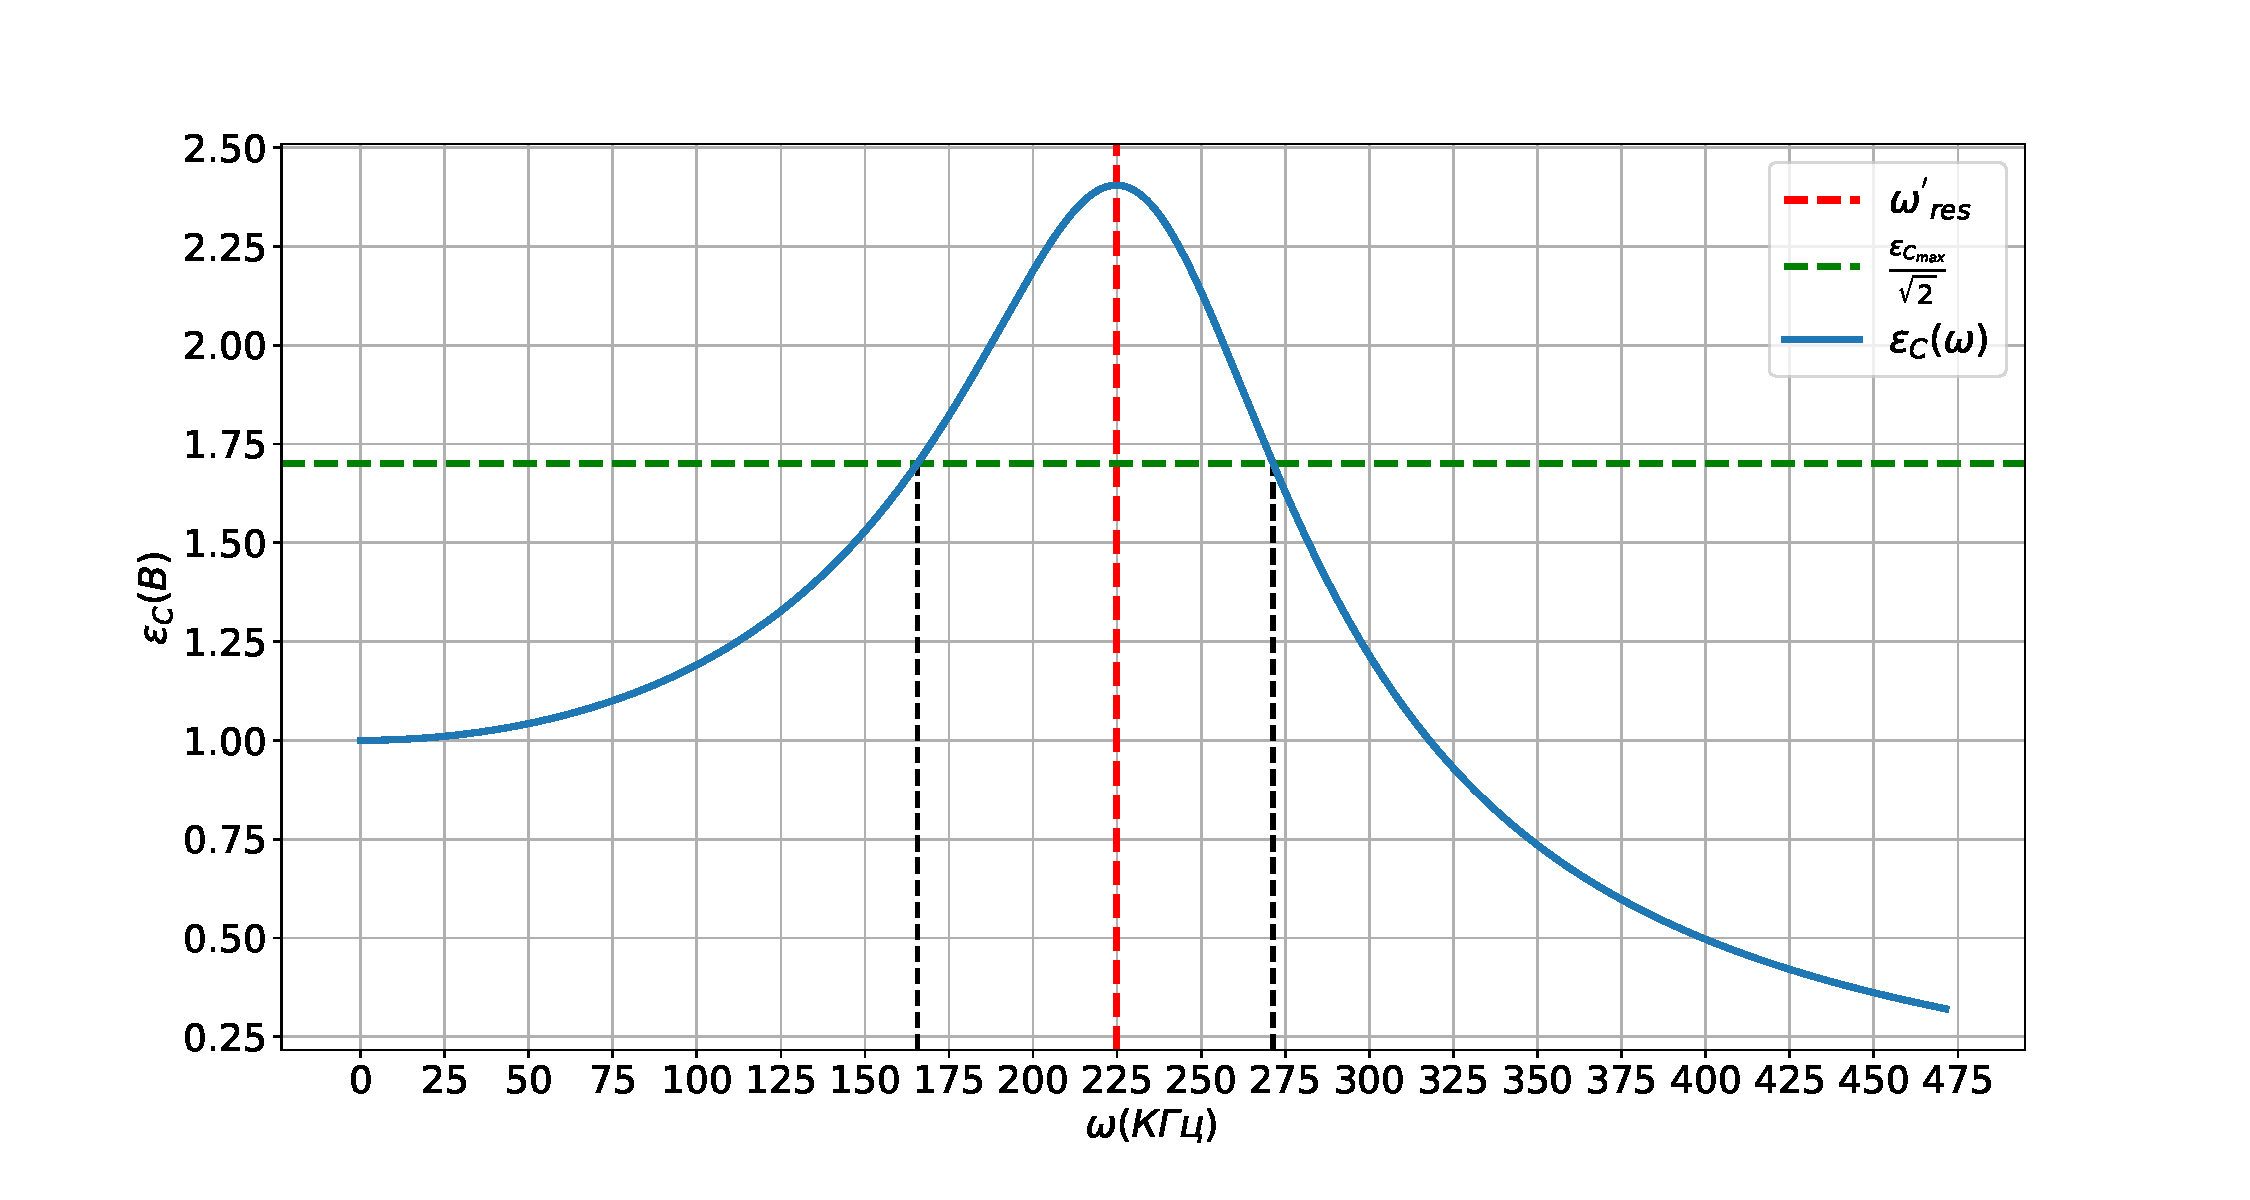
\includegraphics[width=1.0\textwidth]{graphics/EC(w).pdf}

    \item З графіка $\varepsilon_C(\omega)$ визначити добротність контура $Q^{'}$.
    Знайти відносну похибку отриманого значення.

    З графіку визначимо $\Delta \omega^{'} = 105 \times 10^3(c^{-1})$, тоді:
    $$ Q_*^{'} = \frac{\Omega_0}{\Delta \omega^{'}} \simeq 2.4 ,\; \eta = 2.4\%$$


\end{enumerate}

\end{document}